
\documentclass{beamer}

\usepackage{graphicx}

\usetheme{Madrid}
\usecolortheme{default}

\title{05 - Deeplearning and autonomous driving}
\author{Maxime Ellerbach}
\date{March 2023}
\begin{document}

\begin{frame}
    \titlepage
\end{frame}


\begin{frame}{End to End approach}
    \begin{itemize}
        \item Easy to get started
        \item Hard to debug the learned features and their impact on the output prediction
    \end{itemize}
\end{frame}

\begin{frame}{End to End architecture}
    An example of input data
    \begin{itemize}
        \item Image from a camera facing forward
        \item Lidar data
        \item Current speed
        \item Gyroscope
        \item Accelerometer
        \item \ldots
    \end{itemize}

    \centering
    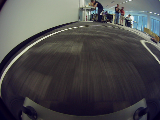
\includegraphics[height=0.4\textheight]{data/real-camera.png}

\end{frame}


\begin{frame}{End to End architecture}
    An example of output data (Labels)
    \begin{itemize}
        \item Steering
        \item Throttle
        \item \ldots
    \end{itemize}
    Here, we are directly predicting the actions the car should take

    \centering
    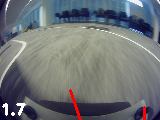
\includegraphics[height=0.4\textheight]{data/left-turn.png}
    
\end{frame}

\begin{frame}{Solving problems separately}
    Instead of directly predicting the throttle, we could split the problem into multiple smaller one:
    \begin{itemize}
        \item Are we currently turning ?
        \item How far is the next turn ?
        \item How fast are we currently going ? Should we go faster ?
    \end{itemize}
    We can then generate a policy which will act better than an estimation of our driving : going faster than human
\end{frame}

\begin{frame}{Architecture of the car}
    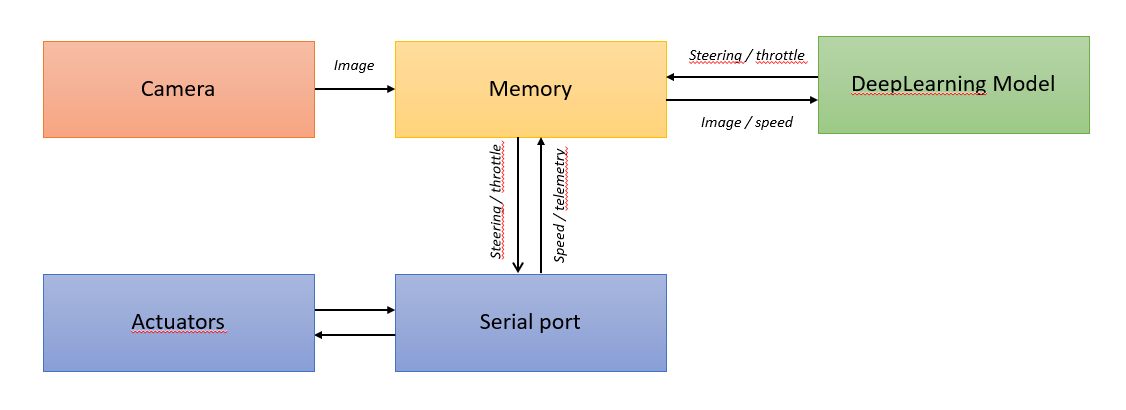
\includegraphics[width=\textwidth]{data/car-control-loop.png}
\end{frame}


\begin{frame}{Practice 03 - Using Donkeycar framework}
    
\end{frame}

\end{document}
